\section{Finite Differences Method for Parabolic PDEs}

\numericsubsection{Richardson's \em{Explicit} FD Scheme}

\begin{enumerate}
	\item \emph{Discretise parabolic PDE} $Lu(...) = f(...)$ using discrete operators
	\item{
		\emph{Discretise geometry} by introducing a grid:
		$x_{j,k} = (j\cdot\Delta x, k\cdot\Delta t)$ with $j$ as the local index
		and $k$ as the time index where $k=0$ is on boundary
		and \colorbox{shadecolor}{$\Delta x = \frac{1}{n}$},
		\colorbox{shadecolor}{$\Delta t = \frac{r}{n^2}$}
		and \colorbox{shadecolor}{$r = \frac{\Delta t}{\Delta x^2}$}
	}
	\item{
		\emph{Introduce approximated nodal values} $\utild(x_{j,k}) = \utild_{j,k}$ and $f_j = f(x_j,0)$ for the Dirichlet boundary conditions.
	}
	\item{
		Find a matrix $C$ that satisfies

		\colorbox{shadecolor}{$
			\displaystyle
			\utild_{j}^{(k+1)}=r\utild_{j-1}^{(k)}+(1-2r)\utild_{j}^{(k)} + r\cdot \utild_{j+1}^{(k)}
		$}

		for inner grid points for each ``step`` satisfying boundary conditions: $\utild_{j}^{(0)}=\utild_{j,0}=f_j$
	}
	\item{
		Iteratively generate solution vector using $\utild^{(k+1)}=C\cdot\utild^{(k)}$
		(i.e. $\utild^{(k)} = C^k\cdot \vec{f}$)
	}
\end{enumerate}

\subsubsection{Stability Analysis}

\begin{wrapfigure}{r}{0.25\columnwidth}
	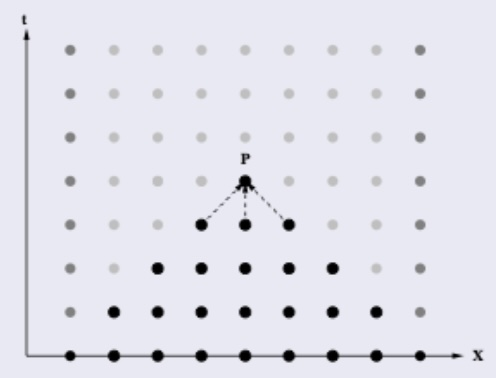
\includegraphics[width=0.25\columnwidth]{images/richardsons}
\end{wrapfigure}

The scheme of Richardson tends asymptotically to zero with k to infinity if
for eigenvalues of $C$, $|\lambda_\mathrm{max}|<1$ is true or $||C^{(n)}||<1$ with respect to the spectral norm of C.

We only receive a good approximation if the steps are small enough to ``catch'' enough information on the boundary.

\subsubsection{Example Using Heat Equation}

\textbf{Given} the heat equation $\frac{\partial u}{\partial t}(x,t) = \frac{\partial^2 u}{\partial x^2}(x,t)$
for the domain $\Omega = [0,1]\times [0, \infty[$ with the boundary conditions
$u(x,0) = e^x$, $u(0,t) = e^t$ and $u(1,t) = e^{1+t}$, we want to find an approximation $\utild$ for points
$(\sfrac{1}{3},\sfrac{2}{3}),(\sfrac{2}{3},\sfrac{2}{3})$ using $\Delta x = \sfrac{1}{3}$ and $\Delta t = \sfrac{1}{3}$.

\textbf{Discretisation of Heat Equation}:
\begin{align*}
	& \frac{u(x,t+\Delta t)-{\color{blue} u(x,t)}}{\color{blue}\Delta t}\approx\frac{u(x+\Delta x,t)-2\cdot u(x,t)+u(x-\Delta x,t)}{\Delta x^{2}} \\
	& u(x,t+\Delta t)\approx {\color{blue}u(x,t)+\Delta t}\cdot{\frac{u(x+\Delta x,t)-2 u(x,t)+u(x-\Delta x,t)}{\Delta x^{2}}} \\
	& \utild_{j,k+1}=u_{j,k}+r\cdot u_{j+1,k} - 2u_{j,k} + u_{j-1,k}\quad {\color{gray}\left|\ r=\frac{\Delta t}{\Delta x^2}\right.} \\
	& \utild_{j,k+1} = r\cdot\utild_{j-1,k}+(1-2r)\utild_{j,k} + r\cdot\utild_{j+1,k}
\end{align*}

\textbf{Discretisation of Geometry}:

\makebox[\columnwidth]{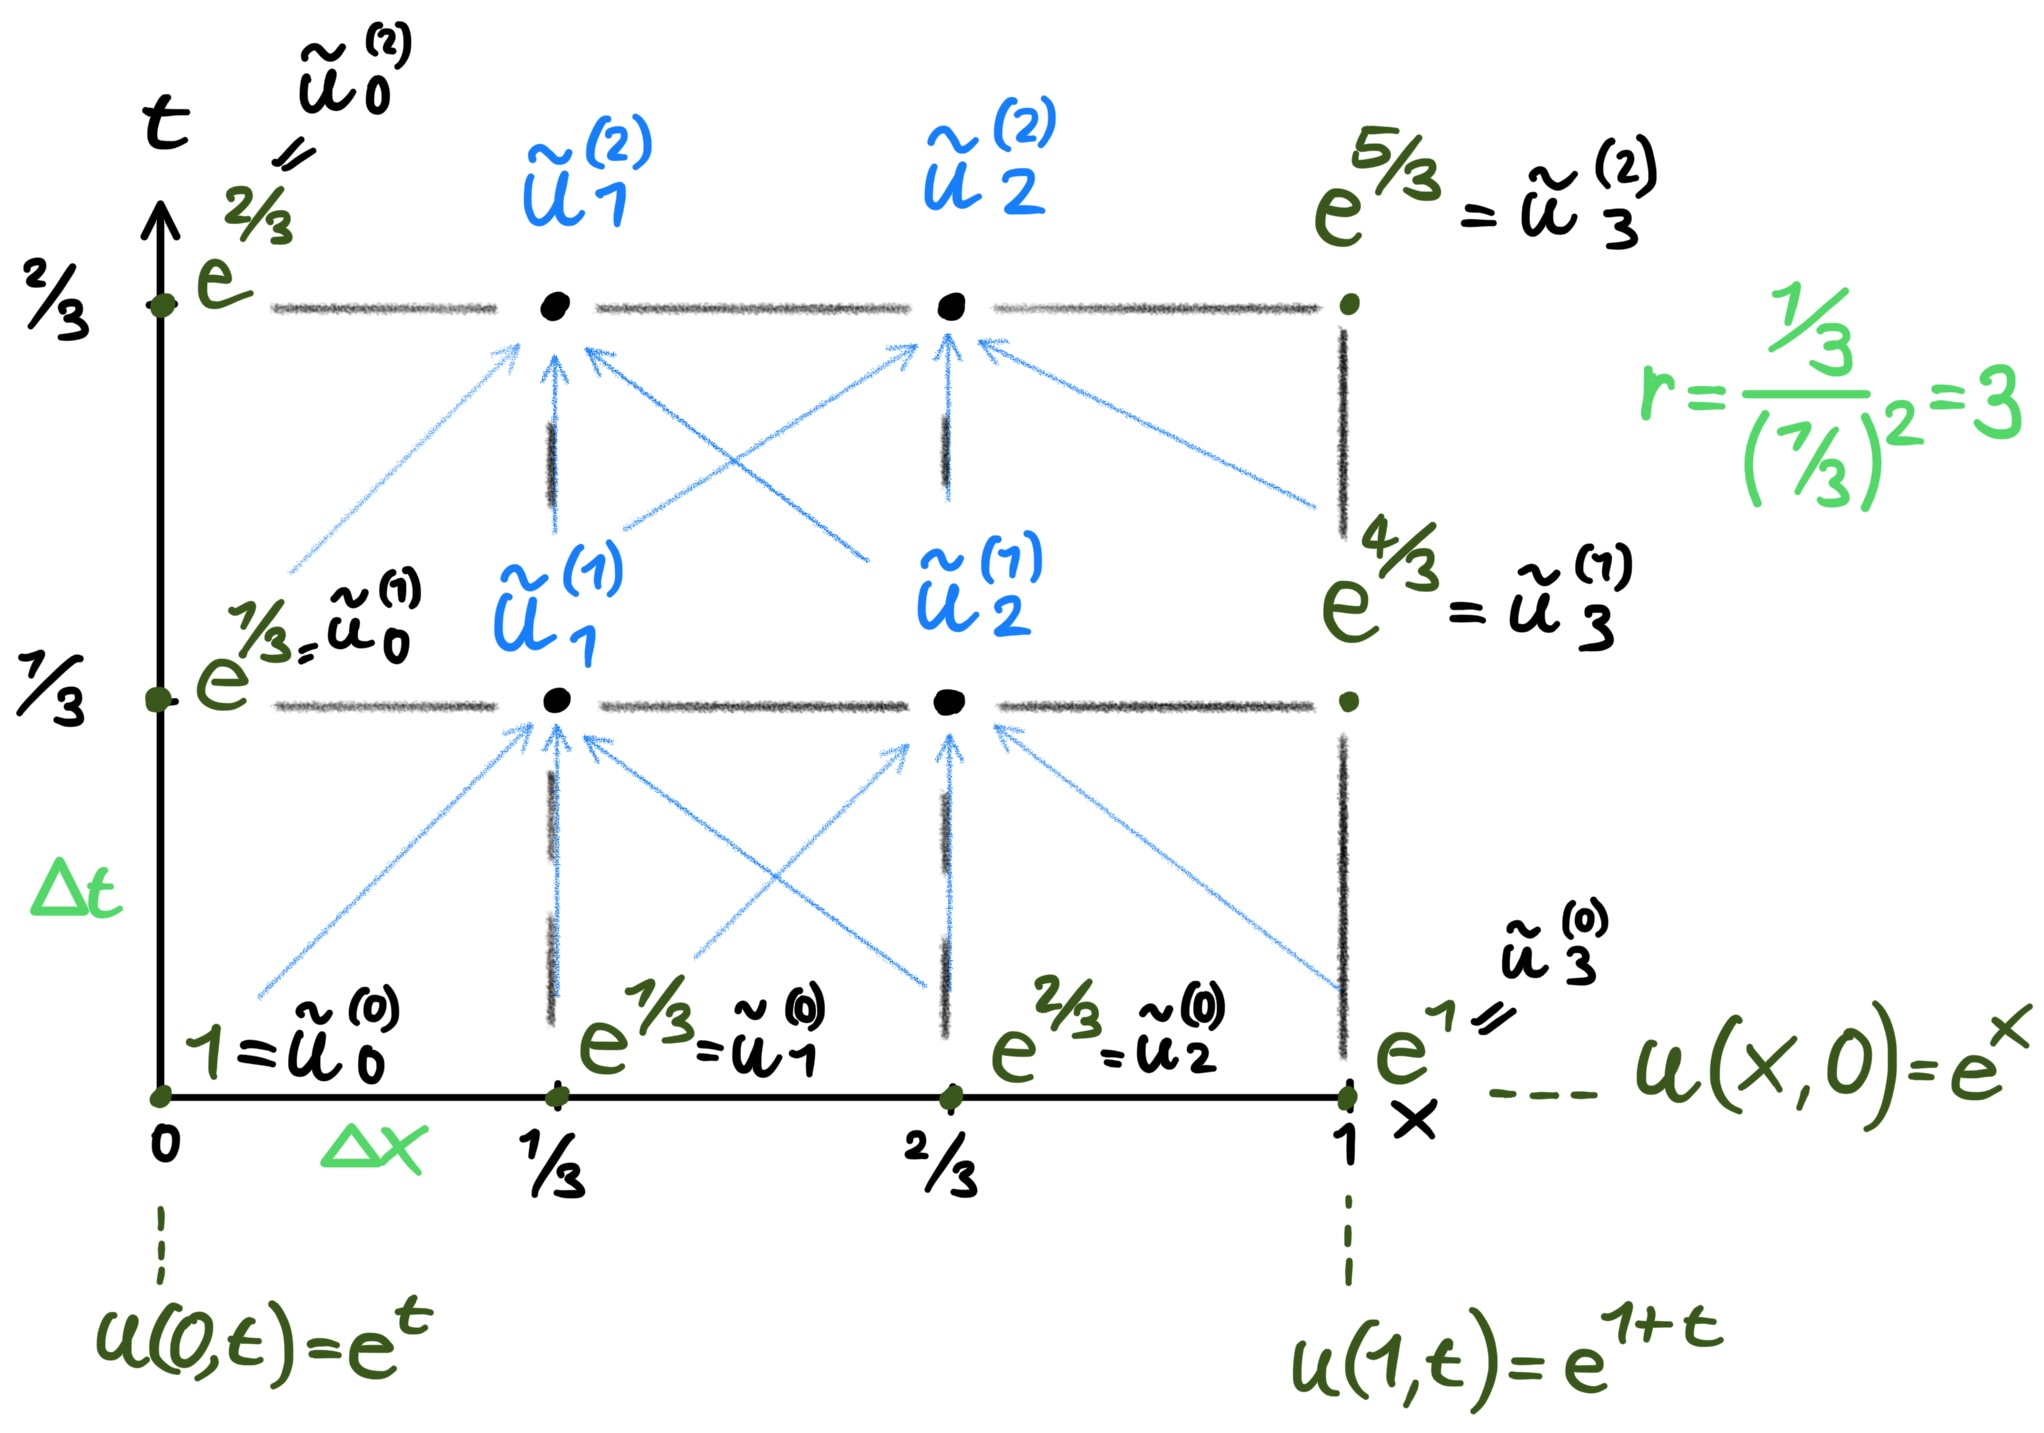
\includegraphics[width=0.75\columnwidth]{images/richardson_explicit}}

\textbf{Solution Method:} With $r$ having a set value, we can write the iterative equation as:
\begin{align*}
	\utild_{j}^{(k+1)} = 3\utild_{j-1}^{(k)} + 5\utild_{j}^{(k)} + 3\utild_{j+1}^{(k)}
\end{align*}

and thus, for $\mathbf{k+1=1}$:
\begin{align*}
	\utild_1^{(1)} & = 3\cancelto{1}{\utild_0^{(0)}} - 5\cancelto{e^{\sfrac{1}{3}}}{\utild_1^{(0)}} + 3\cancelto{e^{\sfrac{2}{3}}}{\utild_2^{(0)}} {\color{gray} = 1.8651} \\
	\utild_2^{(1)} & = 3\utild_1^{(0)} - 5\utild_2^{(0)} + 3\utild_3^{(0)} {\color{gray} = 2.603}
\end{align*}

and $\mathbf{k+1 = 2}$:
\begin{align*}
	\utild_1^{(2)} & = 3\cancelto{e^{\Delta t\cdot k}}{\utild_0^{(1)}} - 5\utild_1^{(1)} + 3\utild_2^{(1)} {\color{gray} = 2.6702} \\
	\utild_2^{(2)} & = 3\utild_1^{(1)} - 5\utild_2^{(1)} + 3\cancelto{e^{1+\Delta t\cdot k}}{\utild_3^{(1)}} {\color{gray} = 3.9614}
\end{align*}

Alternatively, using matrix $C$:
\begin{align*}
	\begin{bmatrix}
		\utild_1 \\
		\utild_2
	\end{bmatrix}^{(k+1)}
	=
	\underbrace{
		\begin{bmatrix}
			-5 & 3 \\
			3 & -5
		\end{bmatrix}
	}_{C}
	\begin{bmatrix}
		\utild_1 \\
		\utild_2
	\end{bmatrix}^{(k)}
	+
	\underbrace{
		3\begin{bmatrix}
			e^{\Delta t k} = e^\frac{k}{3} \\
			e^{1+\Delta t k} = e^{1+\frac{k}{3}}
		\end{bmatrix}
	}_\text{Dirichlet B.C.}
\end{align*}

and
\begin{align*}
	\begin{bmatrix}
		\utild_1 \\
		\utild_2
	\end{bmatrix}^{(2)}
	=
	C^2\vec{\utild}^{(0)} + C\cdot 3\begin{bmatrix}
		1 \\
		e
	\end{bmatrix}
	+
	3\begin{bmatrix}
		e^{\sfrac{1}{3}} \\
		e^{\sfrac{4}{3}}
	\end{bmatrix}
	{\color{gray}
		=
		\begin{bmatrix}
			2.6702 \\
			3.9614
		\end{bmatrix}
	}
\end{align*}

\numericsubsection{Richardson's \em{Implicit} Scheme}

Uses a backward finite difference for the discretisation in $t$:
\begin{align*}
	\frac{\partial u}{\partial t} \approx \frac{u(x,t) - u(x, t-\Delta t)}{\Delta t}
\end{align*}
to be able to consider all boundary points.
We therefore look for a matrix $E$ to receive a system of linear equations:
\begin{align*}
	E\cdot \utild^{(k+1)} = \utild^{(k)}
\end{align*}
and get a solution by inverting (of course not suitable for numerical tasks, only theoretical):
\begin{align*}
	\utild^{(k+1)} = \left(E^{(n)}\right)^{-1}\cdot\utild^{(k)}
\end{align*}

The method is stable independently of $r$ (absolute stability).

\subsubsection{Example}

\textbf{Given} the heat equation $\frac{\partial u}{\partial t}(x,t) = \frac{\partial^2 u}{\partial x^2}(x,t)$
for the domain $\Omega = [0,2]\times [0, \infty[$ with boundary condition
$u(x,0) = \sin\left(\frac{\pi x}{2}\right)$. We want to find $\utild(x,0.1)$ using $\Delta x = 0.5$ and $\Delta t = 0.05$.
\\[1em]
\textbf{Discretisation of Heat Equation}
analogously like in the explicit method:
\begin{align*}
	\tilde{u}_{j}^{(k)}=-r\cdot\utild_{j-1}^{(k+1)}+(1+2\cdot r)\cdot\tilde{u}_{j}^{(k+1)}-r\cdot\tilde{u}_{j+1}^{(k+1)}
\end{align*}

\textbf{Discretisation of Geometry}

\makebox[\columnwidth]{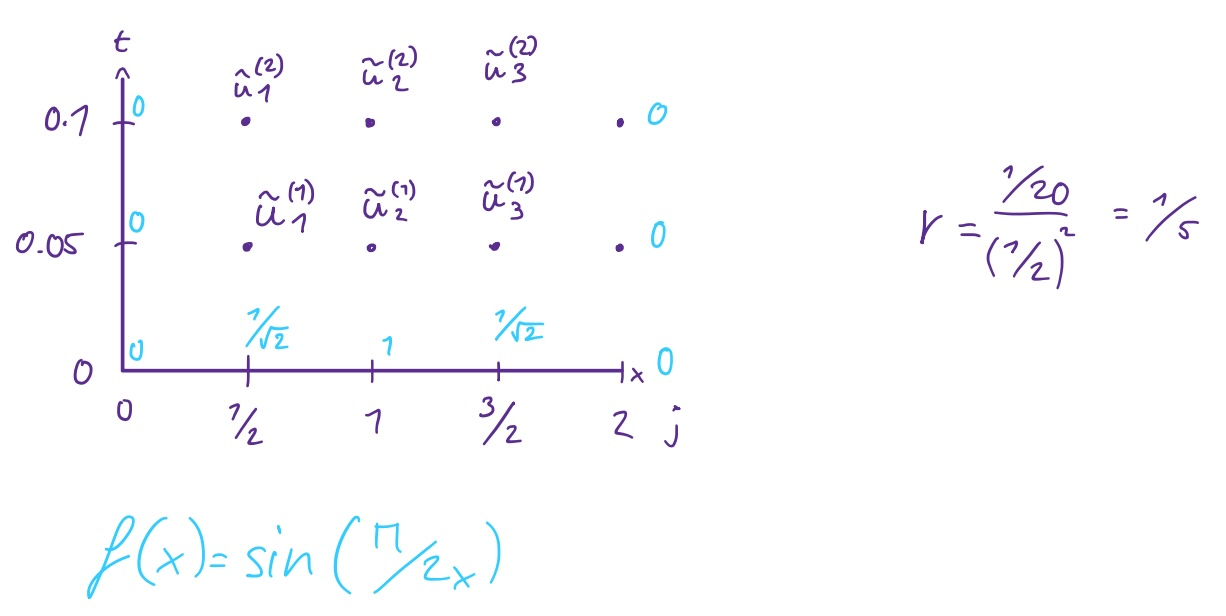
\includegraphics[width=\columnwidth]{images/richardson_implicit}}

\textbf{Solution}

For $k=0$:
\begin{align*}
	\mathbf{j=1} : & -\cancelto{\frac{1}{5}}{r}\cdot\cancelto{\color{cyan}0}{\utild_{0}^{(1)}} + \sfrac{7}{5}\cdot\utild_1^{(1)} - \cancelto{\frac{1}{5}}{r}\cdot\utild_2^{(1)} = f(\sfrac{1}{2}) = {\color{cyan}\sfrac{1}{\sqrt{2}}} \\
	\mathbf{j=2} : & -\cancelto{\frac{1}{5}}{r}\cdot\utild_{1}^{(1)} + \sfrac{7}{5}\cdot\utild_2^{(1)} - \cancelto{\frac{1}{5}}{r}\cdot\utild_3^{(1)} = f(1) = {\color{cyan}1} \\
	\mathbf{j=3} : & -\cancelto{\frac{1}{5}}{r}\cdot\utild_{2}^{(1)} + \sfrac{7}{5}\cdot\utild_3^{(1)} - \cancelto{\frac{1}{5}}{r}\cdot\cancelto{\color{cyan}0}{\utild_4^{(1)}} = f(\sfrac{3}{2}) = {\color{cyan}\sfrac{1}{\sqrt{2}}} \\
\end{align*}

resulting in the linear system
\begin{align*}
	\underbrace{
		\begin{bmatrix}
			\sfrac{7}{5} & -\sfrac{1}{5} & 0 \\
			-\sfrac{1}{5} & \sfrac{7}{5} & -\sfrac{1}{5} \\
			0 & -\sfrac{1}{5} & \sfrac{7}{5}
		\end{bmatrix}
	}_{E}
	\begin{bmatrix}
		\utild_1 \\
		\utild_2 \\
		\utild_3 \\
	\end{bmatrix}^{(1)}
	=
	\begin{bmatrix}
		\sfrac{1}{\sqrt{2}} \\
		1 \\
		\sfrac{1}{\sqrt{2}}
	\end{bmatrix}
	& \Rightarrow
	\begin{bmatrix}
		\utild_1 \\
		\utild_2 \\
		\utild_3 \\
	\end{bmatrix}^{(1)}
	\approxeq
	{\color{purple}
	\begin{bmatrix}
		0.633 \\
		0.895 \\
		0.633
	\end{bmatrix}
	} \\
	\overbrace{
		\begin{bmatrix}
			\sfrac{7}{5} & -\sfrac{1}{5} & 0 \\
			-\sfrac{1}{5} & \sfrac{7}{5} & -\sfrac{1}{5} \\
			0 & -\sfrac{1}{5} & \sfrac{7}{5}
		\end{bmatrix}
	}
	\begin{bmatrix}
		\utild_1 \\
		\utild_2 \\
		\utild_3 \\
	\end{bmatrix}^{(2)}
	= {\color{purple}
	\begin{bmatrix}
		0.633 \\
		0.895 \\
		0.633
	\end{bmatrix}
	}
	& \Rightarrow
	\begin{bmatrix}
		\utild_1 \\
		\utild_2 \\
		\utild_3 \\
	\end{bmatrix}^{(2)}
	\approxeq
	\begin{bmatrix}
		0.567 \\
		0.801 \\
		0.567
	\end{bmatrix}
\end{align*}

\numericsubsection{Crank-Nicolson Scheme}

Averaging the explicit and implicit method of Richardson to improve error term:
\begin{align*}
	g^{\prime}(x)={\frac{1}{2}}\cdot\left({\frac{g(x+\Delta x)-g(x)}{\Delta x}}+{\frac{g(x)-g(x-\Delta x)}{\Delta x}}\right)
	+ \mathcal{O}(\Delta x^{2})
\end{align*}

The Crank-Nicolson values at time-level $k+1$ are computed by solving the system of linear equations
\begin{align*}
	F^{(n)}\cdot\vec{\utild}^{(k+1)} = G^{(n)}\cdot\vec{\utild}^{(k)}
\end{align*}

which can formally be transformed into the linear iteration
\begin{align*}
	\vec{\utild}^{(k+1)}=\left(F^{(n)}\right)^{-1}\cdot G^{(n)}\cdot\vec{\utild}^{(k)}
\end{align*}

where the matrices $F$ and $G$ are for the heat equation $u_t=u_{xx}$:
\begin{align*}
	& F^{(n)}=E^{(n)}+I=\mathrm{tridiag}_{n-1}(-r,2+2\cdot r,-r) \\
	& G^{(n)}=C^{(n)}+I=\mathrm{tridiag}_{n-1}(r,2-2\cdot r,r)
\end{align*}

with
\begin{align*}
	E^{(n)}=\mathrm{tridiag}_{n-1}(-r,1+2\cdot r,-r)	\quad\text{(from implicit)}
\end{align*}
and
\begin{align*}
	C^{(n)}=\mathrm{tridiag}_{n-1}(r,1-2\cdot r,r)\quad\text{(from explicit)}
\end{align*}

\subsubsection{Example}

\textbf{Given} the heat equation $\frac{\partial u}{\partial t}(x,t) = \frac{\partial^2 u}{\partial x^2}(x,t)$
for the domain $\Omega = [0,3]\times [0, \infty[$ and boundary condition
$u(x,0) = -25x^2(x-3)$, we want to find $\utild(x,2)$ using $\Delta x = 1$ and $\Delta t = 0.5$.

\textbf{Discretisation of Geometry}

\makebox[\columnwidth]{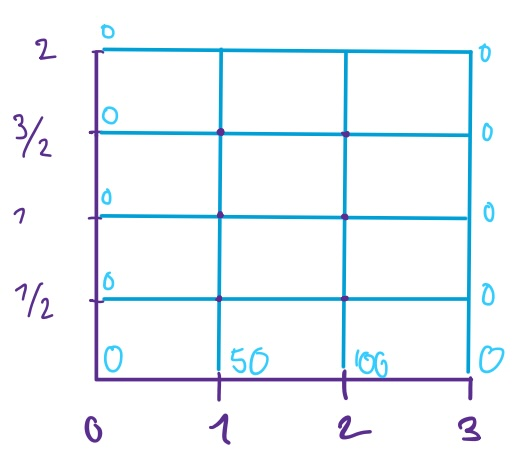
\includegraphics[width=0.4\columnwidth]{images/crank_nicolson}}

\textbf{Solution}

With $r = \frac{\Delta t}{\Delta x^2} = \frac{\sfrac{1}{2}}{1} = 0.5$, we receive the matrices
\begin{align*}
	F = \begin{bmatrix}
		3 & -0.5 \\
		-0.5 & 3
	\end{bmatrix},
	G = \begin{bmatrix}
		1 & 0.5 \\
		0.5 & 1
	\end{bmatrix}
\end{align*}

and thus
\begin{align*}
	\begin{bmatrix}
		\utild_1 \\
		\utild_2
	\end{bmatrix}^{(k+1)}
	=
	F^{-1} G
	\begin{bmatrix}
		\utild_1 \\
		\utild_2
	\end{bmatrix}^{(k)}
	\Rightarrow
	\begin{bmatrix}
		\utild_1 \\
		\utild_2
	\end{bmatrix}^{(4)}
	=
	(F^{-1} G)^4
	\begin{bmatrix}
		\utild_1 = 50 \\
		\utild_2 = 100
	\end{bmatrix}^{(0)}
\end{align*}






